\documentclass[12pt]{article}                           % Document class -- add [12pt] before {article} for 12pt font
\usepackage[letterpaper, margin=1in]{geometry}    % Paper type and margin size
\usepackage[english]{isodate}                     % Sets the date to US style
\usepackage[USenglish]{babel}                     % US English as language
\usepackage[utf8]{inputenc}                       %
\usepackage{amsmath,amsthm,amssymb,amsfonts}      % Math packages
\usepackage[margin=10pt,font=small,labelfont=bf, labelsep=endash]{caption}
\usepackage{longtable}                            % Package for longtables
\usepackage{lscape}                               % Landscape tables
\usepackage{epigraph}                             % Pretty quotes with \epigraph{}
\usepackage{booktabs,calc}
\usepackage{tikz}
\usetikzlibrary{decorations.text,calc,arrows.meta}
\usepackage{graphicx}                             % Allows the import of graphs and figures
\graphicspath{ {images/} }
\usepackage{caption}
\usepackage{subcaption}
\usepackage{pdflscape}
% \pagestyle{empty}
% \usepackage[activate={true,nocompatibility},final,tracking=true,kerning=true,spacing=true,factor=1100,stretch=10,shrink=10]{microtype}
\usepackage{lastpage}                             % For page number in footer
\usepackage{todonotes}                            % To do list in the text
\usepackage{multicol}                             % Multiple columns
\usepackage{natbib}                               % Bibliography package
\setcitestyle{aysep={}}                           % Author Year (no comma)
\usepackage{parskip}                              % No default indent
\usepackage{setspace}                             % Adjust line-spacing
%\singlespacing
% \onehalfspacing
\doublespacing
\usepackage{rotating}                             % Rotate figures and tables
\usepackage{bm}                                  % Use Greek boldface \bm{\beta}
% \microtypecontext{spacing=nonfrench}
\usepackage{float}


\begin{document}

\title{Gift Travel in the U.S. House of Representatives}
\author{Anonymous}
\date{\today}



\maketitle

\thispagestyle{empty}

\newpage
\abstract{The relationship between interest groups and members of Congress plays out in many ways, some of which have received great scholarly attention while others have gone relatively unnoticed. We present a study highlighting the gifted trips that members take at the invitation and reimbursement of nongovernmental organizations. We introduce this "gift travel" as a tool that interest groups use to influence and exchange information with members. We analyze all gift-travel reports provided to the Clerk of the House from 2007 to 2017. Members (and their staff) reported taking 10,364 trips during that time, with each member traveling an average of 4.75 times per biennium. We find that interest groups target powerful members over the rank and file; and that more ideologically extreme members are more likely to go on gifted trips. Our analysis opens a new avenue for research on the interaction between members of Congress and interest groups.}
\thispagestyle{empty}

\newpage
\setcounter{page}{1}
\pagenumbering{arabic}

Gift travel occurs when a member, or one of her staff, goes on an expense-paid trip sponsored by a non-governmental organization, such as a trade association, think tank, cable channel, or university. Going on an expense-paid trip, often over the course of several days, compared to accepting one of hundreds of campaign contributions, is more meaningful for a relationship between a member and an interest group. Time may be a legislator's most important resource \citep[34]{Fenno1978}. When members go on these sponsored trips, they must report it to the Clerk of the House.\footnote{According to Rule XXV, clause 5 of the Rules of the House of Representatives, members must disclose reimbursement for such travel within 15 days of return. The Clerk of the House makes a report of these disclosures public on its website.} Members reported spending 42,388 days on 10,364  gift trips over the 2007-2017 period, with each member traveling an average 19 days per biennium.

Our argument is built upon the scholarship that has failed to find a link between campaign contributions and roll-call votes \citep{Welch1982,Wright1990}. Moreover, we seek to build upon scholarship that has argued for a more nuanced relationship between interest groups and members, like contributions timed before key votes or committee markups \citep{Stratmann1998,Hall1990}, contributions in exchange for meetings with members \citep{Langbein1986}, and the provision of information or services to members' offices \citep{Hall2006}.

This nuanced approach to interest group and member behavior is consistent with previous research on privately sponsored travel. \cite{Rosenson2009} argues that trip sponsors may have multiple goals in sending members on trips and that members have various reasons for accepting their invitations. She finds that institutional power, ideology, and seniority all play a role in predicting trips by members or their staffs \citep{Rosenson2009}. We examine a broader period of activity than Rosenson, though only for House members, and utilize data reported directly to the Clerk of the House instead of to a third party.

While money is generally seen as the most important resource to many politicos, we argue that the scarcity of time on Capitol Hill is of far greater importance due to its scarcity. Any time spent on gifted trips during recess is time not spent in the district;\footnote{Note that occasionally gifted trips occur with state delegations, which may entail members visiting their own districts. Most trips occur outside of members' districts.} and, any time spent while the House is in session needs to be coordinated with leadership to ensure no important votes will be missed. Put simply, gift travel requires much more activity from a member than simply receiving a check. In turn, we argue that interest groups provide members with gift travel as an attempt to buy face-to-face access, reinforce relationships, and support their policy-related activity \citep{Hall2006}.

We theorize that sponsoring organizations seek short-term policy influence, information exchange, and the opportunity to have the member's attention and build a long-term relationship. Therefore, we conjecture that groups target members who are strategically positioned to influence policy. Such members will likely be among the party leadership \citep{Cox2005,Rosenson2009}, electorally safe \citep{Grimmer2013a}, senior \citep{Snyder1992,Rosenson2009}, and relatively moderate ideologically \citep{Alduncin2017}. Sponsors are typically specialized organizations, like trade associations or think tanks, and must balance their preferences for power, policy interest, and feasibility. While everyone might want to get the ear of the Speaker, only the most resourceful sponsors are apt to do so. Others must take what they can get, and use their finances wisely \citep{Barber2017}.

Despite a lack of scholarly attention, gift travel has already been highlighted by the popular media as potentially corrupting. For example, at the end of May 2013, ten members of Congress, along with thirty-two staffers and dozens of state legislators, traveled to Baku, Azerbaijan. Gathering on the shore of the Caspian Sea, they took part in an all-expense-paid conference and cultural visit. The members and their staff listened to speeches given by the president of Azerbaijan, three former advisers to President Obama, and attended at least three briefings pertaining to the country's state-owned oil company. The trip sparked controversy when it was reported that the Azerbaijan-affiliated nonprofits that sponsored the travel had used money originating from a state agent, the very same state-owned oil company that had held information sessions during the conference \citep{Tucker2014}.

While it is legal for nongovernmental organizations to pay for members to go on such excursions, members are forbidden from accepting travel offers from foreign countries or corporations that employ U.S. lobbyists, and members may not meet with lobbyists at any time during their travel \citep{Wickham2015}.

The Baku trip highlights the potential for gift travel to be gamed by the sponsors, the laxness of the self-reporting system, and the difficulty in connecting what goes on during these trips with legislators' preferences and behavior. While this particular trip was unusual because it may have involved breaking federal law, in many other ways it was an ordinary instance of gift travel. Members were invited by a nonprofit to listen to speeches in and tour around a foreign country. The speeches, briefings, and mingling were all a part of what a member typically experiences on a gift-travel trip.

We present three major findings. First, party leaders, committee chairs, and ranking members travel much more than the rank and file, which is consistent with Rosenstone's data from 2001-2004. Second, seniority is not a significant predictor of the number of gift travel trips a member goes on, and electoral safety has only a trivial effect. Third, and unexpectedly, more ideologically extreme members travel more than their moderate colleagues. We will now turn to our data and detail what we know about gift travel. We close the paper with a more detailed discussion of our findings, the implications thereof, and suggestions for avenues of future research on gift travel and corruption in Congress.

\subsection*{Data}

Every year since 2007, the Office of the Clerk of the U.S. House of Representatives has published all gift travel reports. This paper analyzes these reports from the 110th through the 114th Congresses (2007-2017). These data, after cleaning, collapsing duplicate trip entries, and aggregating by member, consist of 2,180 observations, which are at the level of the member per congress. Over the course of the ten-year period for which we have data, each member, or their staff, traveled an average 19 days per congress and reported spending a total of 42,388 days (on 10,364 trips) engaged in gift travel; the average trip is about four days.

After attempting to correct for typos and various names for the same organization, we found that a total of 1,466 nongovernmental sources provided reimbursement for travel to members of Congress between 2007 and 2017.\footnote{Filing these reports is left up to the members and their staffs. It is up to them to spell the name of the sponsor correctly, use the full name or an abbreviation, and, indeed, know exactly who it is that is sponsoring the trip. Because of this, the true number of sponsors is likely slightly lower than 1,466.} Each of these organizations gave at least one gift-trip in that ten-year period, which equates to about 250 organizations per Congress, with each congressional cohort taking about 2,500 trips.

A small number of familiar names are responsible for a hefty portion of the number of trips taken each congress. Only about 4\% (63 out of 1466) of the sponsoring organizations averaged at least one trip per Congress, or five total in the data set. This datum would imply that only five or six dozen organizations are assuming the cost of putting members on trips as a regular part of business. The other 95\% or so appear to be using gift travel only sparingly, possibly in reaction to shifts in the policy agenda or opportunities to alter the policy content of bills \citep{Hall1990}. The sixty-two organizations that, on average, sponsored one or more trips per Congress account for 72\% of the all the reported trips in our data set. The concentration of gifting behavior among a handful of sponsors is an important descriptive fact to note. See Appendix Table 1 for a list of the top travel sponsors.

To get some notion of who the big players are, let's look briefly at the top five sponsors. The most active sponsor, by far, is an organization called the Congressional Institute, which provided travel subsidies an average of 371 occasions per Congress. The Congressional Institute appears to invite great numbers of members, usually around 150 of them, to places near Washington, such as Hot Springs, Virginia. This is the same group that \cite{Rosenson2009} indicated as the top sponsor.

The remaining travel sponsors are the American Israel Education Foundation (146 trips per Congress), the Aspen Institute (107), the Heritage Foundation (88), and the Humpty Dumpty Institute (46). The Aspen Institute and the Heritage Foundation are think tanks; the Humpty Dumpty Institute is an international NGO; and the American Israel Education Foundation is an interest group, self-described as being part of America's pro-Israel lobby.

The dependent variable for our analysis is \emph{trips}. It is a count, i.e., a sum of binary items (traveled or did not), and it is over-dispersed.\footnote{Overdispersion occurs when the observed variance is larger than the expected variance from a given model. The count is the number of separate journeys reported by each member to the Clerk of the House; each unique report counts as one trip.} Further, there is heterogeneity across individuals' probabilities of traveling. We estimate a negative binomial regression using maximum likelihood, and include fixed-effects for each Congress. The full regression results are in Table A1.

Our trips variable is aggregated at the office level. Members do not go on every trip themselves. We argue this aggregation is appropriate because a member's office is instrumental to her legislative behavior \citep{Mayhew1974}, and because sponsors continue to provide travel even though staffers are the ones visiting. The data indicate that members go on only about 30\% of the trips they report; the remaining 70\% are attended by staffers. In fact, the proportion of trips taken by staffers, when broken down by Congress, shows that members are attending fewer and fewer trips each congressional biennium. And, even though members are attending smaller proportions of trips each year, the total number of trips reported each year continues to grow.

Not all members (or their staffers) go on gift travel, but most of them do. Of the 2,180 total members, 292 (13.4\%) did not go on a single trip. Similarly, 253 members (11.6\%) went on exactly one, 42 (11.4\%) went on two, 255 (11.7\%) went on three, with 4.8 trips being the mean. Figure A1 shows a histogram of the number of trips taken by all the members. The figure is heavily right-skewed (mean = 4.8, sd = 4.7, median = 4), with only 30 members total (or 6 per Congress) going on 20 or more trips.

Democrats travel less often, on average, compared to Republicans (see Figure A2). The average number of trips among Democrats is 4.3, but the variance is large ($\sigma^2 = 23.7$). Republicans, on average, go on one more trip than Democrats; their average is 5.2, but again, the variance is large ($\sigma^2 = 20.3$).

Of course, not all trips are the same. Some trips involve foreign travel, while others entail just a quick jaunt into a state bordering the District of Columbia. Twenty-nine percent of all trips, on average, involved travel outside the United States. Figure A4 shows that, with the exception of the 114th Congress, foreign trips are growing in number, as are domestic trips. As suspected, members have a clear preference for taking foreign trips instead of sending their staffers in their place (see Figures A6 and A7). And, their preference has grown stronger over time. Members in the 113th and 114th Congresses attended about half of the foreign trips compared to one-third of foreign trips in the 110th Congress. Conversely, in the 110th, members went on 37\% of all domestic trips; by the 114th, that number had shrunk to 14\%. Over time, offices are going on more total trips, but the members are sending their staffers to many of the domestic destinations.

\subsection*{Results and Discussion}

What characteristics separate those who travel often from those who stay in Washington or only travel to their districts? The predicted counts reported in Table 1 offer answers to this question. The statistically significant parameter estimates for these position-of-power variables---party leaders, committee chairs, and ranking members---indicate that powerful members travel more, but the coefficients alone do not give us a clear idea of how many more trips per Congress they go on. For the substantive meaning of the regression estimates, we calculate predicted number of trips. Holding all other power variables at zero and the continuous variables, \emph{seniority}, \emph{win percentage}, and \emph{ideological extremity}, at their sample means, the effect of being party leader is sizable: a party leader is predicted to go on 5.49 trips per Congress, three more trips than a rank-and-file member, an increase of 113\% (see Table 1). The effect of being a committee chair is almost identical in size to that of being a party leader, while the effect of ranking member differs across party.

\begin{table}[h]
\centering
\caption{Predicted Number of Trips}
\label{}
\begin{tabular}{@{}lll@{}}
\toprule
                            & No                 & Yes                 \\ \midrule
Committee Chair             & 2.58              & 5.52              \\
                            & {[}2.33 - 2.85{]} & {[}4.62 - 6.59{]} \\
Democrat                    & 2.58              & 2.17              \\
                            & {[}2.33 - 2.85{]} & {[}1.97 - 2.39{]} \\
Party Leader                & 2.58              & 5.49              \\
                            & {[}2.33 - 2.85{]} & {[}4.20 - 7.17{]} \\
Ranking Member (Republican) & 2.58              & 4.83              \\
                            & {[}2.33 - 2.85{]} & {[}3.75 - 6.22{]} \\
Ranking Member (Democratic) & 2.17              & 2.49              \\
                            & {[}1.97 - 2.39{]} & {[}1.98 - 3.15{]} \\ \bottomrule
\multicolumn{2}{l}{\footnotesize Note: Standard errors reported in brackets.}    \\
\end{tabular}
\end{table}

The interactive effect of ideological extremity and party on the number of gift-travel trips members go on is the second major finding of this paper. It is important not only because the magnitude of its effect is large but also because it reveals how ideology works to attract sponsors toward members in different degrees depending on their party. The large positive effect of ideological extremity holds for members of both parties, but the size of the effect is larger for Democrats than it is for Republicans. Visualized in Figure 1, the predicted number of trips for Republicans can be seen to rise from 2.1 to 3.3 (57\% increase), while the number for Democrats jumps from 0.9 to 4.8 (433\% increase). So, what a Democrat may lack in committee power in the eyes of sponsors, she may make up for if her views are sufficiently liberal.

\begin{figure}[hbt]
\centering
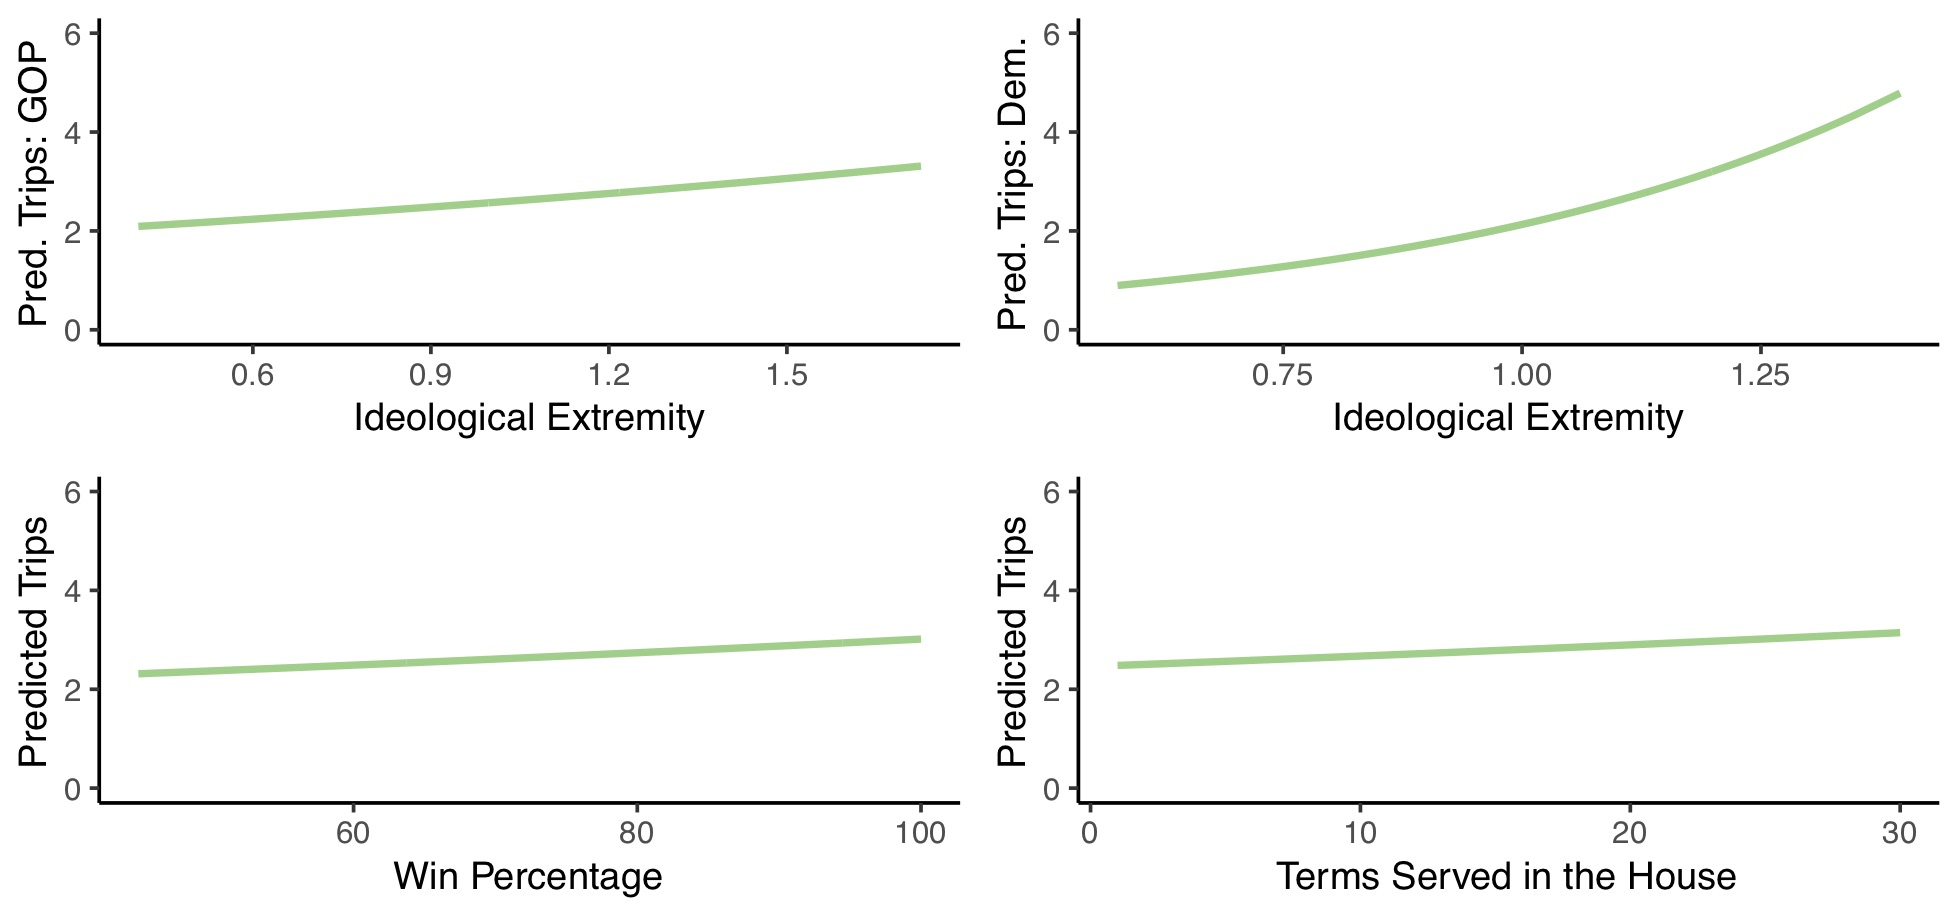
\includegraphics[scale=.6]{fig1.jpeg}
  \caption{Predicted Trips Taken by Member per Congress}
\end{figure}

We also find some interesting null effects and observe two noteworthy trends. First, though we expected otherwise, more senior and electorally safe members are no more likely than their marginal freshman counterparts to take a trip on someone else's dime. Second, since gift travel has been reported in its current fashion, members have only gone on more and more trips per congressional term.

In line with scholarship regarding the travel of members via Congressional Delegations \citep{Alduncin2014,Alduncin2017}, scholars could examine who travels with whom and how often. Future scholarship on member travel should also try to better specify the relationship between sponsors and members. A measure of sponsor ideological similarity would go a good ways in specifying the relationship, as would a coding of committee-related variables. Like sophisticated donors, sponsors may also target the committees most relevant to their policy goals, or ones ideologically similar to them \citep{Barber2017}. Our analysis speaks to who travels and how much, but future work should investigate whether those who travel more do so because they receive trips from a wide variety of sponsors or because they are given trips again and again by the same big organizations.

\newpage

\begin{thebibliography}{xx}

\harvarditem[Alduncin, Parker \harvardand\ Theriault]{Alduncin, Parker
  \harvardand\ Theriault}{2017}{Alduncin2017}
Alduncin, Alexander, David C.~W. Parker \harvardand\ Sean~M. Theriault. 2017.
\newblock ``Leaving on a {{Jet Plane}}: {{Polarization}}, {{Foreign Travel}},
  and {{Comity}} in {{Congress}}.'' {\em Congress \& the Presidency} pp.~1--24.

\harvarditem[Alduncin et~al.]{Alduncin, Kelly, Parker \harvardand\
  Theriault}{2014}{Alduncin2014}
Alduncin, Alexander, Sean~Q. Kelly, David C.~W. Parker \harvardand\ Sean~M.
  Theriault. 2014.
\newblock ``Foreign {{Junkets}} or {{Learning}} to {{Legislate}}?
  {{Generational Changes}} in the {{International Travel Patterns}} of {{House
  Members}}, 1977-2012.'' {\em The Forum} 12(3).

\harvarditem[Barber, {Canes-Wrone} \harvardand\ Thrower]{Barber, {Canes-Wrone}
  \harvardand\ Thrower}{2017}{Barber2017}
Barber, Michael~J., Brandice {Canes-Wrone} \harvardand\ Sharece Thrower. 2017.
\newblock ``Ideologically {{Sophisticated Donors}}: {{Which Candidates Do
  Individual Contributors Finance}}?'' {\em American Journal of Political
  Science} 61(2):271--288.

\harvarditem{Cox \harvardand\ McCubbins}{2005}{Cox2005}
Cox, Gary \harvardand\ Matthew McCubbins. 2005.
\newblock {\em Setting the {{Agenda}}: {{Responsible Party Government}} in the
  {{U}}.{{S}}. {{House}} of {{Representatives}}}.
\newblock New York:  {University of Cambridge Press}.

\harvarditem{Fenno}{1978}{Fenno1978}
Fenno, Richard. 1978.
\newblock {\em Home {{Style}}: {{House Members}} in {{Their Districts}}}.
\newblock New York:  {HarperCollins}.

\harvarditem{Grimmer}{2013}{Grimmer2013a}
Grimmer, Justin. 2013.
\newblock ``Appropriators Not {{Position Takers}}: {{The Distorting Effects}}
  of {{Electoral Incentives}} on {{Congressional Representation}}.'' {\em
  American Journal of Political Science} 57(3):624--642.

\harvarditem{Hall \harvardand\ Deardorff}{2006}{Hall2006}
Hall, Richard~L. \harvardand\ Alan~V. Deardorff. 2006.
\newblock ``Lobbying as {{Legislative Subsidy}}.'' {\em American Political
  Science Review} 100(01):69--84.

\harvarditem{Hall \harvardand\ Wayman}{1990}{Hall1990}
Hall, Richard~L. \harvardand\ Frank~W. Wayman. 1990.
\newblock ``Buying {{Time}}: {{Moneyed Interests}} and the {{Mobilization}} of
  {{Bias}} in {{Congressional Committees}}.'' {\em American Political Science
  Review} 84(3):797.

\harvarditem{Langbein}{1986}{Langbein1986}
Langbein, Laura~I. 1986.
\newblock ``Money and {{Access}}: {{Some Empirical Evidence}}.'' {\em The
  Journal of Politics} 48(4):1052--1062.

\harvarditem{Mayhew}{1974}{Mayhew1974}
Mayhew, David. 1974.
\newblock {\em Congress: {{The Electoral Connection}}}.
\newblock New Haven:  {Yale University Press}.

\harvarditem{Rosenson}{2009}{Rosenson2009}
Rosenson, Beth~A. 2009.
\newblock ``Congressional {{Frequent Flyers}}: {{Demand}}-and {{Supply}}-{{Side
  Explanations}} for {{Privately Sponsored Travel}}.'' {\em Legislative Studies
  Quarterly} 34(2):245--271.

\harvarditem{Snyder}{1992}{Snyder1992}
Snyder, James~M. 1992.
\newblock ``Long-{{Term Investing}} in {{Politicians}}; {{Or}}, {{Give Early}},
  {{Give Often}}.'' {\em Journal of Law \& Economics} 35(April):15--44.

\harvarditem{Stratmann}{1998}{Stratmann1998}
Stratmann, Thomas. 1998.
\newblock ``The Market for Congressional Votes: {{Is}} Timing of Contributions
  Everything?'' {\em The Journal of Law and Economics} 41(1):85--114.

\harvarditem{Tucker \harvardand\ Olsen}{2014}{Tucker2014}
Tucker, Will \harvardand\ Lise Olsen. 2014.
\newblock ``Lawmakers' Trips to {{Baku}} Conference Raise Ethics Questions.''
  {\em Houston Chronicle} .

\harvarditem{Welch}{1982}{Welch1982}
Welch, W.~P. 1982.
\newblock ``Campaign {{Contributions}} and {{Legislative Voting}}: {{Milk
  Money}} and {{Dairy Price Supports}}.'' {\em The Western Political Quarterly}
  35(4):478.

\harvarditem{Wickham}{2015}{Wickham2015}
Wickham, Thomas~J. 2015.
\newblock {\em Constitution, {{Jefferson}}'s {{Manual}}, and {{Rules}} of the
  {{House}} of the {{Representatives}} of the {{United States One Hundred
  Fourteenth Congress}}}.
\newblock Washington, D.C.:  {U.S. Government Publishing Office}.

\harvarditem{Wright}{1990}{Wright1990}
Wright, John~R. 1990.
\newblock ``Contributions, {{Lobbying}}, and {{Committee Voting}} in the
  {{U}}.{{S}}. {{House}} of {{Representatives}}.'' {\em American Political
  Science Review} 84(2):417.

\end{thebibliography}

\newpage







\end{document}
